\documentclass[11pt]{article}
\input{\string~/.macros}
\usepackage[a4paper, total={7in, 9in}]{geometry}
\usepackage{bbm}
\usepackage{mathrsfs} % really cursive alphabets
\usepackage{graphicx}
    \graphicspath{{./assets}}
\usepackage{hyperref}
    \hypersetup{colorlinks=true, linktoc=all, linkcolor=blue, citecolor=red}
\usepackage[backend=bibtex,sorting=none]{biblatex}
\usepackage[margin=0cm]{caption}

% random variables
\newcommand\ry{\ensuremath{\mathsf{y}}}
\newcommand\rx{\ensuremath{\mathsf{x}}}
\newcommand\rb{\ensuremath{\mathsf{b}}} 
\newcommand\rc{\ensuremath{\mathsf{c}}}
\newcommand\rz{\ensuremath{\mathsf{z}}}
\newcommand\ru{\ensuremath{\mathsf{u}}}
\newcommand\rw{\ensuremath{\mathsf{w}}}
\newcommand\rpa{\ensuremath{\mathsf{pa}}}
\newcommand\rU{\ensuremath{\mathsf{U}}}
\newcommand\rbx{\ensuremath{\mathsf{\mathbf{x}}}}
\newcommand\rby{\ensuremath{\mathsf{\mathbf{y}}}}
\newcommand\rbu{\ensuremath{\mathsf{\mathbf{u}}}}

\newcommand\bbP{\ensuremath{\mathbbm{P}}}
\newcommand\bbQ{\ensuremath{\mathbbm{Q}}}


% boldsymbols
\renewcommand\bmu{\ensuremath{\boldsymbol{\mu}}}
\newcommand\bSigma{\ensuremath{\boldsymbol{\Sigma}}}
\newcommand\bgamma{\ensuremath{\boldsymbol{\gamma}}}
\newcommand\bomega{\ensuremath{\boldsymbol{\omega}}}
\newcommand\bnu{\ensuremath{\boldsymbol{\nu}}}


% optimization, classes of functions
\newcommand\scrF{\ensuremath{\mathscr{F}}}
\newcommand\scrS{\ensuremath{\mathscr{S}}}
\newcommand\scrP{\ensuremath{\mathscr{P}}}

% independence
\newcommand{\dperp}{\ensuremath{\perp\!\!\!\perp}}
\newcommand{\ndperp}{\ensuremath{\not\!\perp\!\!\!\perp}}

% operators
\newcommand{\prox}{\ensuremath{\mathsf{prox}}}
\addbibresource{GP.bib}

\begin{document}
 
\section{Gaussian Process}

\cite{carledwardrasmussenGaussianProcessMachine2006} introduces Gaussian Process regression as an alternative view to Bayesian regression. 

\subsection{Bayesian Regression}
 
In linear regression setup, we assume output $y\in\R$ is a linear function of inputs $x\in\R^d$, corrupted with additive iid normal noise,
\begin{align}
    y = f(x) + \epsilon
    \quad\text{where}\quad
    f(x) = w^Tx
    \quad\text{and}\quad
    \epsilon \sim \sN(0, \sigma_n^2)
\end{align}
The Bayesian setup considers $w\in\R^d$ as a random variable, endowed with prior $w\sim \sN(0,\Sigma_p)$. Using Bayes rule, we can find the posterior of weights given data, which is again a normal random variable $p(w \mid X, y) = \sN\left(w \; ; A^{-1}b, A^{-1} \right)$ where $A=\frac{1}{\sigma_n^2} X^TX + \Sigma_p^{-1}$ and $b = \frac{1}{\sigma_n^2}X^Ty$ and $X\in\R^{n\times d}, y\in\R^{n\times 1}$ are design matrices. For test point $x_*$, the predictive distribution of $f_*=f(x_*)$ is the average likelihood of $f_*$ under model $f(x;w)$ with respect to posterior of $w$.
\begin{align}
    p(f_*\mid x_*, X, y)
        = \int p(f_*\mid x_*,w) p(w\mid X, y) \, dw
    \label{eq:kernel_bayesian_regression_predictive_distribution_integral}
\end{align}
We can think of the predictive distribution as a linear function $f_* = x_*^Tw$ of weights, a normal random variable, and therefore is normal. Therefore, $f_*\mid x_*,X,y \sim \sN( x_*^T A^{-1}b, x_*^T A^{-1}x_* )$. The natural extension to Bayesian linear regression is to kernelize it, for example assume a linear model in some feature space $f(x) = \phi(x)^Tw$ for some feature map $\phi:\R^d\to\R^D$. We can write predictive distribution as 
\begin{align}
    f_* \mid x_*,X,y \sim \sN(
        & k(x_*,X) (k(X,X)+\sigma_n^2 I)^{-1}y, \\
        & k(x_*,x_*) - k(x_*,X)(k(X,X) + \sigma_n^2 I)^{-1} k(X,x_*))
    \label{eq:kernel_bayesian_regression_predictive_distribution}
\end{align}
where $k(X,X') = \Phi \Sigma_p \Phi'^T \in \R^{n\times n'}$ and $\Phi\in\R^{n\times D}$ are the feature vectors.

\subsection{Gaussian Process}


\begin{definition}
    (Gaussian Process) A Gaussian process is a stochastic process $\pc{X_t}_{t\in T}$ such that, for every finite subset of indices $t_1,\cdots,t_k \in T$, $(X_{t_1},\cdots,X_{t_k})$ is multivariate normal.
\end{definition}

A Gaussian process $f\sim \sG\sP(m,k)$ over $\R^{\sX}$ is fully specified by the mean function $m:\sX\to\R$ and covariance function $k:\sX\times\sX\to\R$ where
\begin{align}
    m(x)=\E\pb{f(x)}
    \quad\quad\quad
    k(x,x') = \E\pb{ (f(x)-m(x))(f(x')-m(x')) }
\end{align}
The covariance function determines function's behavior, for example its stationarity, smoothness, and periodicity etc. For example, the squared exponential covariance function $k_{\text{SE}}(x,x') = \exp( -\frac{1}{2\ell^2} \norm{x-x'}_2^2 )$ enforces the prior knowledge that functions are smooth, i.e. inputs are close in the Euclidean sense will have similar outputs. See Figure (\ref{fig:plt_sample_from_gp}) for some examples of samples from Gaussian process.

\begin{example}
    (Intuition about covariance matrix for $\sG\sP$) First consider $(y_1,y_2) \sim \sN(\mathbf{0}, \Sigma)$ where $\Sigma_{11}=\Sigma_{22} = 1$ and $\Sigma_{12}=\Sigma_{21}=\rho_{12}$. We know $y_1\mid y_2 = a \sim \sN(\rho_{12} a, 1 -  \rho_{12}^2)$. When $\cov(y_1,y_2) = \rho_{12} \uparrow 1$, $y_1$'s samples conditioned on $y_2=a$ fall close to $a$ with high probability. When $\rho_{12} \downarrow 0$, $y_1 \mid y_2=a$ will distribute like a unit normal, regardless of values that $y_2$ take. Extend this intuition to gaussian process: whenever $k(x_i,x_j)$ is large, $y_i,y_j$ are correlated and so observing $y_i=a$ provides a strong prior on how $y_j$ will behave, or in other words, reduce the uncertainty of values that $y_j$ can take dramatically.
\end{example}


\begin{center} 
\begin{figure}[h!]
    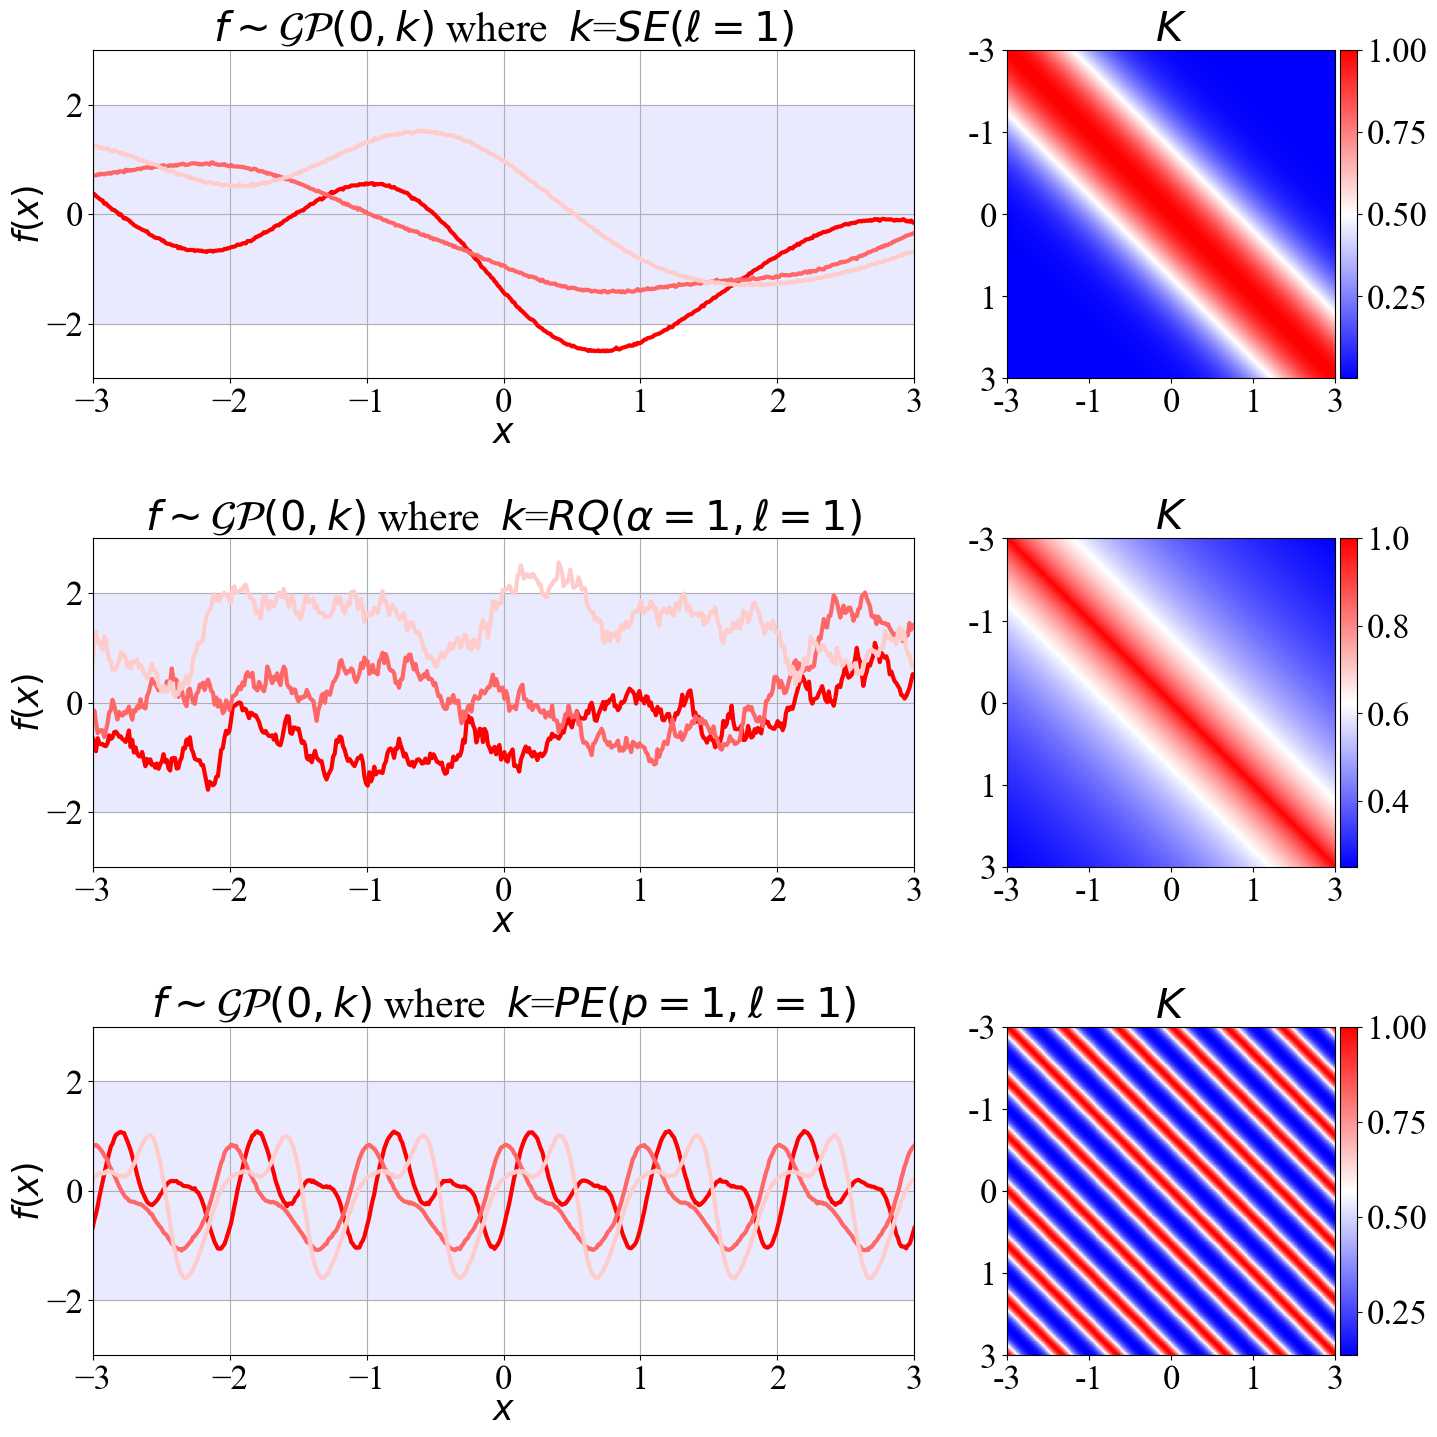
\includegraphics[width=\textwidth]{assets/plt_sample_from_gp.png} 
    \caption{(Left) Samples from Gaussian process prior and (Right) covariance matrix at test locations.}
    \label{fig:plt_sample_from_gp}
\end{figure}
\end{center} 
    

\subsection{Gaussian Process Regression}

Instead of placing a prior over weights $p(w)$ to quantify randomness in function $f(x)=\phi(x)^Tw$, we model function directly as a Gaussian process, $f\sim \sG\sP(0,k)$. There is a one-to-one correspondence between the two views. For example, $f(x)=\phi(x)^Tw$ with prior $w\sim \sN(0,\Sigma_p)$ used in kernel Bayesian regression has
\begin{align}
    \E\pb{f(x)}
        = \phi(x)^T \E\pb{w} = 0
    \quad\quad\quad
    \E\pb{ f(x)f(x') }
        = \phi(x)^T\Sigma_p \phi(x')
\end{align}
Therefore, $f\sim \sG\sP(0, k)$ where $k(x,x') = \phi(x)^T \Sigma_p \phi(x')$. Note $k$ is in fact a valid kernel. (Since $\Sigma_p$ is psd, $\Sigma_p = UDU^T$ by SVD. We can write $k(x,x') = \inner{\psi(x)}{\psi(x')}$ where $\psi(x) = \Sigma_p^{1/2} \phi(x)$ and $\Sigma_p^{1/2} = UD^{1/2}U^T$). Conversely, any valid kernel used in kernel Bayesian regression can be used to parameterize the covariance function of the Gaussian process model over $f$.

Since $y=f(x)+\epsilon$, we have $\by = \mathbf{f} + \sigma_n^2 I \sim \sN(0, k(X,X)+\sigma_n^2I)$ where $\by,\mathbf{f}\in\R^{n\times 1}$. We can write the joint distribution of observed values and function values at some test locations $X_*$ as
\begin{align}
    \begin{bmatrix}
        \by \\ \mathbf{f}_*
    \end{bmatrix}
    \sim
    \sN\left(
        \mathbf{0},
        \begin{bmatrix}
            k(X,X) + \sigma_n^2I & k(X,X_*) \\
            k(X_*,X) & k(X_*,X_*) \\ 
        \end{bmatrix}
    \right)
    \label{eq:gaussian_process_regression_noisy_model}
\end{align}
We can derive the predictive distribution for $\mathbf{f}_*\mid \by$ by simply apply conditional distribution formula
\begin{align}
    \mathbf{f}_* \mid X,\by, X_* \sim \sN(
        & k(X_*,X) (k(X,X)+\sigma_n^2 I)^{-1} \by  \\
        & k(X_*,X_*) - k(X_*,X) (k(X,X)+\sigma_n^2 I)^{-1} k(X,X_*) )
    \label{eq:gp_regression_predictive_distribution}
\end{align}
which has exact form compared to (\ref{eq:kernel_bayesian_regression_predictive_distribution}). More compactly, for a single test point $x_*$, $\mu_{\mathbf{f}_*} =  k_*^T (K+\sigma_n^2 I)^{-1}$ and $\var(\mathbf{f}_*) = k(x_*,x_*) - k_*^T (K+\sigma_n^2 I)^{-1} k_* $ where $k_* = k(X,x_*)\in \R^{n\times 1}$. See Figure (\ref{fig:plt_gp_regression_inference}) for examples of Gaussian process regression with varying data size and hyperparameters. 


\begin{center} 
\begin{figure}[h!]
    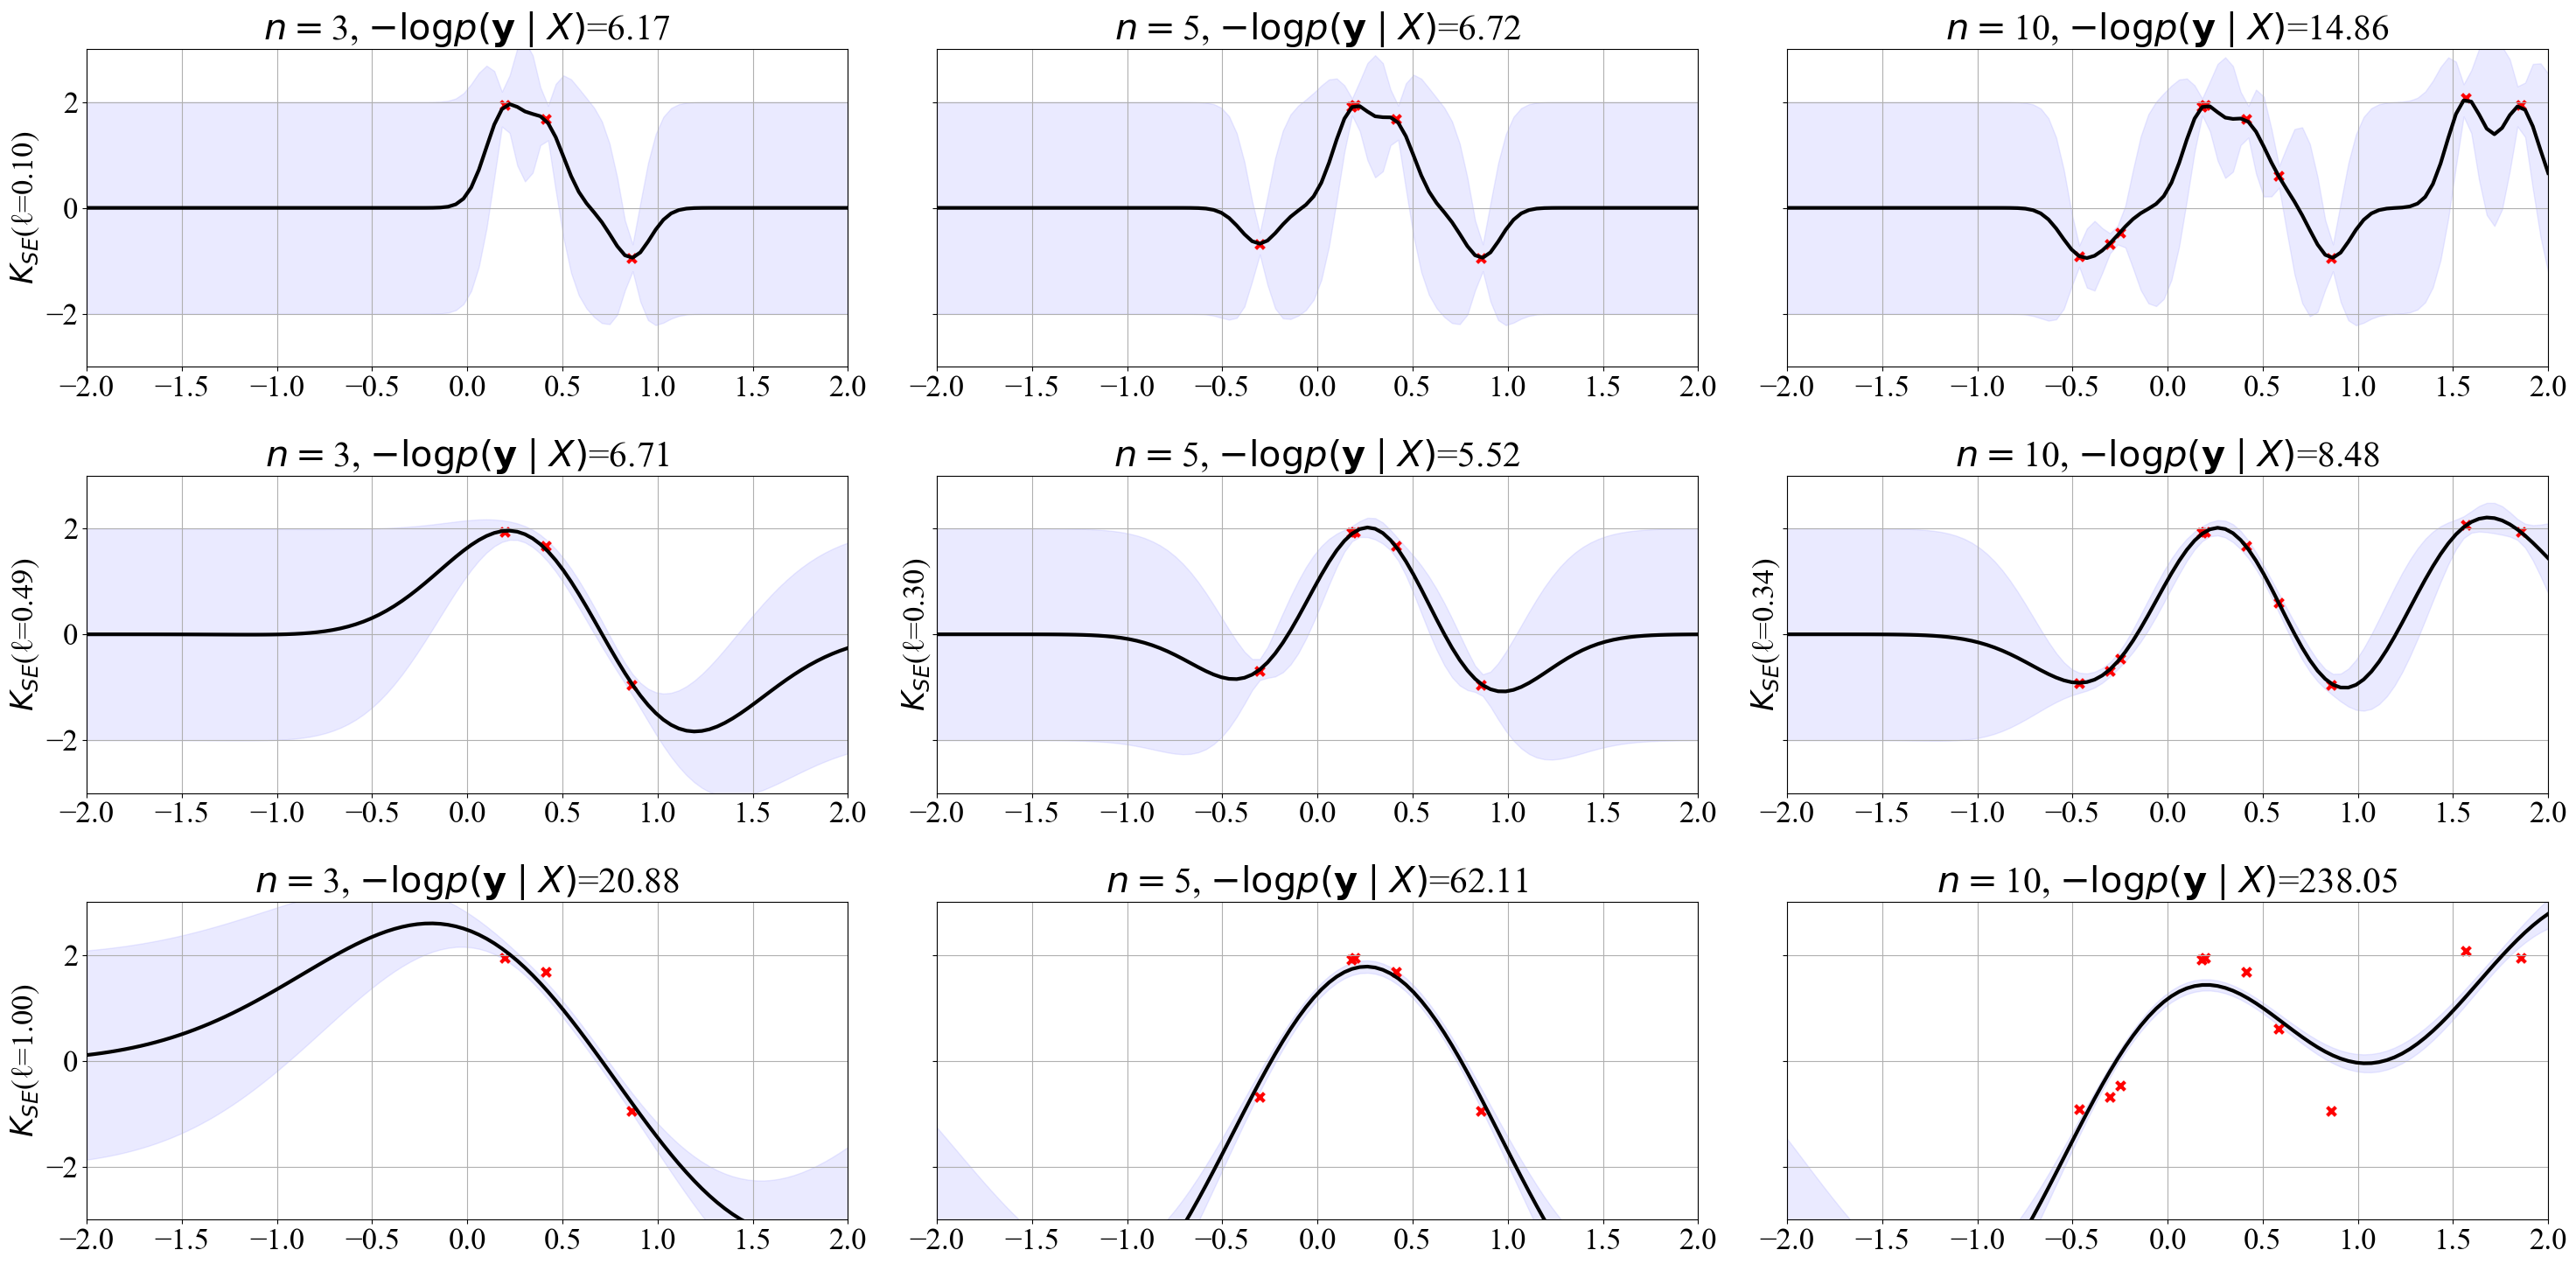
\includegraphics[width=\textwidth]{assets/plt_gp_regression_inference.png} 
    \caption{This plot shows mean (black) and 95\% confidence interval (light blue) for predictive distribution $p(\mathbf{f}_*\mid X,\by, X_*)$ fit using Gaussian process regression assuming a SE prior over $f\sim\sG\sP(0,k_{SE})$ of varying lengthscale $\ell$ and observed sample sizes $n$. The middle row's kernel hyperparameter is taken to be $\ell = \argmax p(\by\mid X, \ell)$, optimized via gradient descent}
    \label{fig:plt_gp_regression_inference}
\end{figure}
\end{center}

\subsection{Model Selection}

Model selection for Gaussian process regression involves picking the form and the hyperparameters of the covariance function.

Given data $(X,\by)$, marginal likelihood $p(\by\mid X)$ quantifies how likely data is observed under our additive noise model $\by\mid \mathbf{f} \sim \sN(\mathbf{f},\sigma_n^2 I)$ on average with respect to latent function values (or parameters of our model) $\mathbf{f}\mid X \sim \sN(0,K)$ (due to assumption of Gaussian process prior over f),
\begin{align}
    p(\by\mid X)
        = \int p(\by\mid \mathbf{f},X) p(\mathbf{f}\mid X) \, d\mathbf{f}
\end{align}
This formulation is analogous to that in Bayesian linear regression where the marginal likelihood marginalizes over weights $p(\by\mid X) = \int p(\by\mid X,w)p(w) \, dw$. We can obtain a closed form expression by reading off (\ref{eq:gaussian_process_regression_noisy_model}), i.e. $\by \sim \sN(\mathbf{0}, K+\sigma_n^2 I)$. In empirical Bayes setup, kernel hyperparameters can be found by maximizing log marginal likelihood,
\begin{align}
    \log p(\by\mid X)
        = -\frac{1}{2} \by^T  (K+\sigma_n^2 I)^{-1}\by - \frac{1}{2} \log |K+\sigma_n^2I| - \frac{n}{2} \log 2\pi 
\end{align}


 


\newpage
\printbibliography 




\end{document}